\documentclass[twoside]{book}

% Packages required by doxygen
\usepackage{fixltx2e}
\usepackage{calc}
\usepackage{doxygen}
\usepackage[export]{adjustbox} % also loads graphicx
\usepackage{graphicx}
\usepackage[utf8]{inputenc}
\usepackage{makeidx}
\usepackage{multicol}
\usepackage{multirow}
\PassOptionsToPackage{warn}{textcomp}
\usepackage{textcomp}
\usepackage[nointegrals]{wasysym}
\usepackage[table]{xcolor}

% Font selection
\usepackage[T1]{fontenc}
\usepackage[scaled=.90]{helvet}
\usepackage{courier}
\usepackage{amssymb}
\usepackage{sectsty}
\renewcommand{\familydefault}{\sfdefault}
\allsectionsfont{%
  \fontseries{bc}\selectfont%
  \color{darkgray}%
}
\renewcommand{\DoxyLabelFont}{%
  \fontseries{bc}\selectfont%
  \color{darkgray}%
}
\newcommand{\+}{\discretionary{\mbox{\scriptsize$\hookleftarrow$}}{}{}}

% Page & text layout
\usepackage{geometry}
\geometry{%
  a4paper,%
  top=2.5cm,%
  bottom=2.5cm,%
  left=2.5cm,%
  right=2.5cm%
}
\tolerance=750
\hfuzz=15pt
\hbadness=750
\setlength{\emergencystretch}{15pt}
\setlength{\parindent}{0cm}
\setlength{\parskip}{3ex plus 2ex minus 2ex}
\makeatletter
\renewcommand{\paragraph}{%
  \@startsection{paragraph}{4}{0ex}{-1.0ex}{1.0ex}{%
    \normalfont\normalsize\bfseries\SS@parafont%
  }%
}
\renewcommand{\subparagraph}{%
  \@startsection{subparagraph}{5}{0ex}{-1.0ex}{1.0ex}{%
    \normalfont\normalsize\bfseries\SS@subparafont%
  }%
}
\makeatother

% Headers & footers
\usepackage{fancyhdr}
\pagestyle{fancyplain}
\fancyhead[LE]{\fancyplain{}{\bfseries\thepage}}
\fancyhead[CE]{\fancyplain{}{}}
\fancyhead[RE]{\fancyplain{}{\bfseries\leftmark}}
\fancyhead[LO]{\fancyplain{}{\bfseries\rightmark}}
\fancyhead[CO]{\fancyplain{}{}}
\fancyhead[RO]{\fancyplain{}{\bfseries\thepage}}
\fancyfoot[LE]{\fancyplain{}{}}
\fancyfoot[CE]{\fancyplain{}{}}
\fancyfoot[RE]{\fancyplain{}{\bfseries\scriptsize Generated by Doxygen }}
\fancyfoot[LO]{\fancyplain{}{\bfseries\scriptsize Generated by Doxygen }}
\fancyfoot[CO]{\fancyplain{}{}}
\fancyfoot[RO]{\fancyplain{}{}}
\renewcommand{\footrulewidth}{0.4pt}
\renewcommand{\chaptermark}[1]{%
  \markboth{#1}{}%
}
\renewcommand{\sectionmark}[1]{%
  \markright{\thesection\ #1}%
}

% Indices & bibliography
\usepackage{natbib}
\usepackage[titles]{tocloft}
\setcounter{tocdepth}{3}
\setcounter{secnumdepth}{5}
\makeindex

% Hyperlinks (required, but should be loaded last)
\usepackage{ifpdf}
\ifpdf
  \usepackage[pdftex,pagebackref=true]{hyperref}
\else
  \usepackage[ps2pdf,pagebackref=true]{hyperref}
\fi
\hypersetup{%
  colorlinks=true,%
  linkcolor=blue,%
  citecolor=blue,%
  unicode%
}

% Custom commands
\newcommand{\clearemptydoublepage}{%
  \newpage{\pagestyle{empty}\cleardoublepage}%
}

\usepackage{caption}
\captionsetup{labelsep=space,justification=centering,font={bf},singlelinecheck=off,skip=4pt,position=top}

%===== C O N T E N T S =====

\begin{document}

% Titlepage & ToC
\hypersetup{pageanchor=false,
             bookmarksnumbered=true,
             pdfencoding=unicode
            }
\pagenumbering{alph}
\begin{titlepage}
\vspace*{7cm}
\begin{center}%
{\Large R\+C\+AC C++ }\\
\vspace*{1cm}
{\large Generated by Doxygen 1.8.13}\\
\end{center}
\end{titlepage}
\clearemptydoublepage
\pagenumbering{roman}
\tableofcontents
\clearemptydoublepage
\pagenumbering{arabic}
\hypersetup{pageanchor=true}

%--- Begin generated contents ---
\chapter{Main Page}
\label{index}\hypertarget{index}{}\begin{DoxyVerb}    ____  _________   ______
   / __ \/ ____/   | / ____/
  / /_/ / /   / /| |/ /     
 / _, _/ /___/ ___ / /___   
/_/ |_|\____/_/  |_\____/   \end{DoxyVerb}
 This is the A\+PI documentation for the Retrospective Cost Adaptive Control (\hyperlink{class_r_c_a_c}{R\+C\+AC}) algorithm.

Take a look at the \hyperlink{_getting_started}{getting started} page to learn how to write your first program with \hyperlink{class_r_c_a_c}{R\+C\+AC}. \begin{DoxyVerb}                          /\
                         /
                        /
            +------------------+            +------------------+
            |                  |            |                  |
            |                  |            |                  |
+---------->+       RCAC       +----------->+                  +------+------->
|           |                  |            |                  |      |
|           |                  |            |                  |      |
|           +------------------+            +------------------+      |
|                /                                                    |
|               /                                                     |
|              /                                                      |
|             /                                                       |
+---------------------------------------------------------------------+
\end{DoxyVerb}
 
\chapter{R\+C\+A\+C\+\_\+cpp}
\label{md__r_e_a_d_m_e}
\Hypertarget{md__r_e_a_d_m_e}
Cpp library implementation of the \hyperlink{class_r_c_a_c}{R\+C\+AC} algorithm

Documentation is through Doxygen and located here \href{https://mohseninima.github.io/RCAC_cpp}{\tt https\+://mohseninima.\+github.\+io/\+R\+C\+A\+C\+\_\+cpp} 
\chapter{Hierarchical Index}
\section{Class Hierarchy}
This inheritance list is sorted roughly, but not completely, alphabetically\+:\begin{DoxyCompactList}
\item \contentsline{section}{R\+C\+AC}{\pageref{class_r_c_a_c}}{}
\begin{DoxyCompactList}
\item \contentsline{section}{R\+C\+A\+C\+Cumgrad}{\pageref{class_r_c_a_c_cumgrad}}{}
\item \contentsline{section}{R\+C\+A\+C\+Grad}{\pageref{class_r_c_a_c_grad}}{}
\item \contentsline{section}{R\+C\+A\+C\+R\+LS}{\pageref{class_r_c_a_c_r_l_s}}{}
\end{DoxyCompactList}
\item \contentsline{section}{rcac\+Cumgrad\+Flags}{\pageref{structrcac_cumgrad_flags}}{}
\item \contentsline{section}{rcac\+Filt}{\pageref{structrcac_filt}}{}
\item \contentsline{section}{rcac\+Flags}{\pageref{structrcac_flags}}{}
\item \contentsline{section}{rcac\+Grad\+Flags}{\pageref{structrcac_grad_flags}}{}
\item \contentsline{section}{rcac\+Rls\+Flags}{\pageref{structrcac_rls_flags}}{}
\end{DoxyCompactList}

\chapter{Class Index}
\section{Class List}
Here are the classes, structs, unions and interfaces with brief descriptions\+:\begin{DoxyCompactList}
\item\contentsline{section}{\hyperlink{class_r_c_a_c}{R\+C\+AC} }{\pageref{class_r_c_a_c}}{}
\item\contentsline{section}{\hyperlink{structrcac_filt}{rcac\+Filt} }{\pageref{structrcac_filt}}{}
\item\contentsline{section}{\hyperlink{structrcac_flags}{rcac\+Flags} }{\pageref{structrcac_flags}}{}
\item\contentsline{section}{\hyperlink{class_r_c_a_c_r_l_s}{R\+C\+A\+C\+R\+LS} }{\pageref{class_r_c_a_c_r_l_s}}{}
\item\contentsline{section}{\hyperlink{structrcac_rls_flags}{rcac\+Rls\+Flags} }{\pageref{structrcac_rls_flags}}{}
\end{DoxyCompactList}

\chapter{File Index}
\section{File List}
Here is a list of all documented files with brief descriptions\+:\begin{DoxyCompactList}
\item\contentsline{section}{{\bfseries R\+C\+A\+C.\+hpp} }{\pageref{_r_c_a_c_8hpp}}{}
\item\contentsline{section}{\hyperlink{_r_c_a_c_creator_8hpp}{R\+C\+A\+C\+Creator.\+hpp} }{\pageref{_r_c_a_c_creator_8hpp}}{}
\item\contentsline{section}{{\bfseries R\+C\+A\+C\+R\+L\+S.\+hpp} }{\pageref{_r_c_a_c_r_l_s_8hpp}}{}
\end{DoxyCompactList}

\chapter{Class Documentation}
\hypertarget{class_r_c_a_c}{}\section{R\+C\+AC Class Reference}
\label{class_r_c_a_c}\index{R\+C\+AC@{R\+C\+AC}}


{\ttfamily \#include $<$R\+C\+A\+C.\+hpp$>$}



Inheritance diagram for R\+C\+AC\+:\nopagebreak
\begin{figure}[H]
\begin{center}
\leavevmode
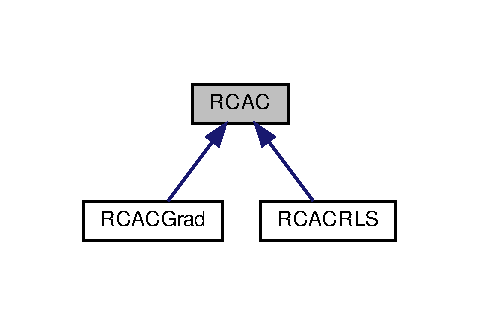
\includegraphics[width=230pt]{class_r_c_a_c__inherit__graph}
\end{center}
\end{figure}


Collaboration diagram for R\+C\+AC\+:\nopagebreak
\begin{figure}[H]
\begin{center}
\leavevmode
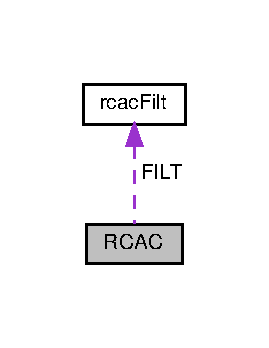
\includegraphics[width=129pt]{class_r_c_a_c__coll__graph}
\end{center}
\end{figure}
\subsection*{Public Member Functions}
\begin{DoxyCompactItemize}
\item 
void \hyperlink{class_r_c_a_c_a956bb6a557f050d3808d5392fd3add20}{one\+Step} (Eigen\+::\+Vector\+Xd \&u\+In, Eigen\+::\+Vector\+Xd \&z\+In, Eigen\+::\+Vector\+Xd \&y\+In)
\item 
Eigen\+::\+Vector\+Xd \hyperlink{class_r_c_a_c_ad93e5753d1810d7c3b2f6fbf56857a51}{get\+Control} ()
\item 
Eigen\+::\+Vector\+Xd \hyperlink{class_r_c_a_c_a5223fc3dbd1a3b4b1577dfd83af76f7e}{get\+Coeff} ()
\item 
int \hyperlink{class_r_c_a_c_ae854b722c35cb1d8506ddacf6a89f795}{getlu} ()
\item 
int \hyperlink{class_r_c_a_c_a1066229fd21de368018ae43747f34622}{getly} ()
\item 
int \hyperlink{class_r_c_a_c_a80a0a753247f22bea53bc5c0b76403a1}{getlz} ()
\item 
int \hyperlink{class_r_c_a_c_a5e3d7aedab3b39415315f1c6b1920ef0}{get\+Nc} ()
\item 
int \hyperlink{class_r_c_a_c_a4e710eaf32fac967dc76a8d851a51211}{getkk} ()
\end{DoxyCompactItemize}
\subsection*{Static Public Member Functions}
\begin{DoxyCompactItemize}
\item 
{\footnotesize template$<$typename T $>$ }\\static \hyperlink{class_r_c_a_c}{R\+C\+AC} $\ast$ \hyperlink{class_r_c_a_c_af7b7133b676886d5010be725291c1a1d}{init} (T \&F\+L\+A\+GS, \hyperlink{structrcac_filt}{rcac\+Filt} \&F\+I\+LT, std\+::string \&which\+R\+C\+AC)
\end{DoxyCompactItemize}
\subsection*{Protected Member Functions}
\begin{DoxyCompactItemize}
\item 
virtual void \hyperlink{class_r_c_a_c_a5ac60fc4b359cf5555427bd1652d6ca1}{coeff\+Update} (Eigen\+::\+Vector\+Xd \&z\+In)=0
\item 
void \hyperlink{class_r_c_a_c_a8dd38159eccbe85cbee4118020c90c88}{init\+Regressor} ()
\item 
void \hyperlink{class_r_c_a_c_aac17e469acf0f2457941d18ae02bfe07}{init\+Filtered} ()
\item 
void \hyperlink{class_r_c_a_c_a5e6bc7050ced3b1be7d9060d089dccfb}{compute\+Filtered} ()
\end{DoxyCompactItemize}
\subsection*{Protected Attributes}
\begin{DoxyCompactItemize}
\item 
\mbox{\Hypertarget{class_r_c_a_c_a92ae57de3b80c8249ee3a328592f3d06}\label{class_r_c_a_c_a92ae57de3b80c8249ee3a328592f3d06}} 
int {\bfseries lz}
\item 
\mbox{\Hypertarget{class_r_c_a_c_aee0473f7ce8fa6a82bb5adddc48577fc}\label{class_r_c_a_c_aee0473f7ce8fa6a82bb5adddc48577fc}} 
int {\bfseries ly}
\item 
\mbox{\Hypertarget{class_r_c_a_c_a6683eb31916f2ee9cbcf1d36d0f382e6}\label{class_r_c_a_c_a6683eb31916f2ee9cbcf1d36d0f382e6}} 
int {\bfseries lu}
\item 
\mbox{\Hypertarget{class_r_c_a_c_ac5e3bbd73052a1a888db85ad89b40d2a}\label{class_r_c_a_c_ac5e3bbd73052a1a888db85ad89b40d2a}} 
int {\bfseries Nc}
\item 
\mbox{\Hypertarget{class_r_c_a_c_af63e5f8e3fd6ab9a896c5b07d572fe5e}\label{class_r_c_a_c_af63e5f8e3fd6ab9a896c5b07d572fe5e}} 
int {\bfseries k\+\_\+0}
\item 
\mbox{\Hypertarget{class_r_c_a_c_aff47c54eac89ed52c2bdd836376d7eed}\label{class_r_c_a_c_aff47c54eac89ed52c2bdd836376d7eed}} 
Eigen\+::\+Vector\+Xd {\bfseries theta\+\_\+0}
\item 
\mbox{\Hypertarget{class_r_c_a_c_a71d835fb0f8e32eab92832bf3a966155}\label{class_r_c_a_c_a71d835fb0f8e32eab92832bf3a966155}} 
int {\bfseries filtorder}
\item 
\mbox{\Hypertarget{class_r_c_a_c_a02f30c9c5a9af4d84de16e1e027489f4}\label{class_r_c_a_c_a02f30c9c5a9af4d84de16e1e027489f4}} 
\hyperlink{structrcac_filt}{rcac\+Filt} {\bfseries F\+I\+LT}
\item 
\mbox{\Hypertarget{class_r_c_a_c_ab087087d4dad63a40fbd7ead4b850c8c}\label{class_r_c_a_c_ab087087d4dad63a40fbd7ead4b850c8c}} 
std\+::deque$<$ Eigen\+::\+Vector\+Xd $>$ {\bfseries u\+Bar}
\item 
\mbox{\Hypertarget{class_r_c_a_c_a6eb81be8397d5605773db459d912f90d}\label{class_r_c_a_c_a6eb81be8397d5605773db459d912f90d}} 
std\+::deque$<$ Eigen\+::\+Vector\+Xd $>$ {\bfseries uf\+Bar}
\item 
\mbox{\Hypertarget{class_r_c_a_c_a06799c662a4c8203f642e17f8c86d33b}\label{class_r_c_a_c_a06799c662a4c8203f642e17f8c86d33b}} 
std\+::deque$<$ Eigen\+::\+Vector\+Xd $>$ {\bfseries z\+Bar}
\item 
\mbox{\Hypertarget{class_r_c_a_c_a774f6216c9c24390701d09c4630dc95d}\label{class_r_c_a_c_a774f6216c9c24390701d09c4630dc95d}} 
std\+::deque$<$ Eigen\+::\+Vector\+Xd $>$ {\bfseries zf\+Bar}
\item 
\mbox{\Hypertarget{class_r_c_a_c_a083bb4d49144a9820f28f637c8ba6eb5}\label{class_r_c_a_c_a083bb4d49144a9820f28f637c8ba6eb5}} 
std\+::deque$<$ Eigen\+::\+Matrix\+Xd $>$ {\bfseries Phi\+Bar}
\item 
\mbox{\Hypertarget{class_r_c_a_c_aa59f73c94933eeb7ade8f8d45533feb1}\label{class_r_c_a_c_aa59f73c94933eeb7ade8f8d45533feb1}} 
std\+::deque$<$ Eigen\+::\+Matrix\+Xd $>$ {\bfseries Phif\+Bar}
\item 
\mbox{\Hypertarget{class_r_c_a_c_ad6bc8005d9983494ee607b697cd85ed7}\label{class_r_c_a_c_ad6bc8005d9983494ee607b697cd85ed7}} 
Eigen\+::\+Matrix\+Xd {\bfseries P}
\item 
\mbox{\Hypertarget{class_r_c_a_c_a06851b7327e7c9095da5e8525dc84889}\label{class_r_c_a_c_a06851b7327e7c9095da5e8525dc84889}} 
Eigen\+::\+Vector\+Xd {\bfseries theta}
\item 
\mbox{\Hypertarget{class_r_c_a_c_a7c1ba0823d931007e737fc77b9489543}\label{class_r_c_a_c_a7c1ba0823d931007e737fc77b9489543}} 
Eigen\+::\+Vector\+Xd {\bfseries u\+Out}
\item 
\mbox{\Hypertarget{class_r_c_a_c_a9759ecd4b93ba787d029f08f92340f08}\label{class_r_c_a_c_a9759ecd4b93ba787d029f08f92340f08}} 
Eigen\+::\+Vector\+Xd {\bfseries u\+In}
\item 
\mbox{\Hypertarget{class_r_c_a_c_a0779330dae6494cfbc0c35c777ab9ba0}\label{class_r_c_a_c_a0779330dae6494cfbc0c35c777ab9ba0}} 
Eigen\+::\+Matrix\+Xd {\bfseries Phi}
\item 
\mbox{\Hypertarget{class_r_c_a_c_a958fc9610d01f86f345238dffc88d925}\label{class_r_c_a_c_a958fc9610d01f86f345238dffc88d925}} 
Eigen\+::\+Vector\+Xd {\bfseries uphi}
\item 
\mbox{\Hypertarget{class_r_c_a_c_af6ed65d38af325245d6857f4a709e1a5}\label{class_r_c_a_c_af6ed65d38af325245d6857f4a709e1a5}} 
Eigen\+::\+Vector\+Xd {\bfseries yphi}
\item 
\mbox{\Hypertarget{class_r_c_a_c_a3502183205d4805bcb23c470adedc998}\label{class_r_c_a_c_a3502183205d4805bcb23c470adedc998}} 
bool {\bfseries rcac\+R\+LS}
\item 
\mbox{\Hypertarget{class_r_c_a_c_acc23e081e96a8fd2dccccc8d0c0b7cdd}\label{class_r_c_a_c_acc23e081e96a8fd2dccccc8d0c0b7cdd}} 
bool {\bfseries rcac\+Grad}
\item 
\mbox{\Hypertarget{class_r_c_a_c_ae965d44ced29623c260b51b4be928b77}\label{class_r_c_a_c_ae965d44ced29623c260b51b4be928b77}} 
int {\bfseries kk} = 1
\end{DoxyCompactItemize}


\subsection{Detailed Description}
The parent \hyperlink{class_r_c_a_c}{R\+C\+AC} class. This class handles all the low level computation of \hyperlink{class_r_c_a_c}{R\+C\+AC} such as the filtering, coefficient updates, and keeping track of the regressors.

Almost all the methods are polymorphic and can be modified by child classes to create \hyperlink{class_r_c_a_c}{R\+C\+AC} algorithms with more complex filtering. 

\subsection{Member Function Documentation}
\mbox{\Hypertarget{class_r_c_a_c_a5ac60fc4b359cf5555427bd1652d6ca1}\label{class_r_c_a_c_a5ac60fc4b359cf5555427bd1652d6ca1}} 
\index{R\+C\+AC@{R\+C\+AC}!coeff\+Update@{coeff\+Update}}
\index{coeff\+Update@{coeff\+Update}!R\+C\+AC@{R\+C\+AC}}
\subsubsection{\texorpdfstring{coeff\+Update()}{coeffUpdate()}}
{\footnotesize\ttfamily virtual void R\+C\+A\+C\+::coeff\+Update (\begin{DoxyParamCaption}\item[{Eigen\+::\+Vector\+Xd \&}]{z\+In }\end{DoxyParamCaption})\hspace{0.3cm}{\ttfamily [protected]}, {\ttfamily [pure virtual]}}

Abstract function for the ceofficient update implementation (e.\+g. R\+LS, Gradient). Child classes must implement this function for \hyperlink{class_r_c_a_c}{R\+C\+AC} to work


\begin{DoxyParams}{Parameters}
{\em z\+In} & performance measurement \\
\hline
\end{DoxyParams}
\mbox{\Hypertarget{class_r_c_a_c_a5e6bc7050ced3b1be7d9060d089dccfb}\label{class_r_c_a_c_a5e6bc7050ced3b1be7d9060d089dccfb}} 
\index{R\+C\+AC@{R\+C\+AC}!compute\+Filtered@{compute\+Filtered}}
\index{compute\+Filtered@{compute\+Filtered}!R\+C\+AC@{R\+C\+AC}}
\subsubsection{\texorpdfstring{compute\+Filtered()}{computeFiltered()}}
{\footnotesize\ttfamily void R\+C\+A\+C\+::compute\+Filtered (\begin{DoxyParamCaption}{ }\end{DoxyParamCaption})\hspace{0.3cm}{\ttfamily [protected]}}

Compute the filtered variables given current regressors and filter values \mbox{\Hypertarget{class_r_c_a_c_a5223fc3dbd1a3b4b1577dfd83af76f7e}\label{class_r_c_a_c_a5223fc3dbd1a3b4b1577dfd83af76f7e}} 
\index{R\+C\+AC@{R\+C\+AC}!get\+Coeff@{get\+Coeff}}
\index{get\+Coeff@{get\+Coeff}!R\+C\+AC@{R\+C\+AC}}
\subsubsection{\texorpdfstring{get\+Coeff()}{getCoeff()}}
{\footnotesize\ttfamily Eigen\+::\+Vector\+Xd R\+C\+A\+C\+::get\+Coeff (\begin{DoxyParamCaption}{ }\end{DoxyParamCaption})\hspace{0.3cm}{\ttfamily [inline]}}

Returns a vector of the current \hyperlink{class_r_c_a_c}{R\+C\+AC} coefficients. \mbox{\Hypertarget{class_r_c_a_c_ad93e5753d1810d7c3b2f6fbf56857a51}\label{class_r_c_a_c_ad93e5753d1810d7c3b2f6fbf56857a51}} 
\index{R\+C\+AC@{R\+C\+AC}!get\+Control@{get\+Control}}
\index{get\+Control@{get\+Control}!R\+C\+AC@{R\+C\+AC}}
\subsubsection{\texorpdfstring{get\+Control()}{getControl()}}
{\footnotesize\ttfamily Eigen\+::\+Vector\+Xd R\+C\+A\+C\+::get\+Control (\begin{DoxyParamCaption}{ }\end{DoxyParamCaption})\hspace{0.3cm}{\ttfamily [inline]}}

Returns \hyperlink{class_r_c_a_c}{R\+C\+AC}\textquotesingle{}s computed value for the control. Must run one\+Step at least once. \mbox{\Hypertarget{class_r_c_a_c_a4e710eaf32fac967dc76a8d851a51211}\label{class_r_c_a_c_a4e710eaf32fac967dc76a8d851a51211}} 
\index{R\+C\+AC@{R\+C\+AC}!getkk@{getkk}}
\index{getkk@{getkk}!R\+C\+AC@{R\+C\+AC}}
\subsubsection{\texorpdfstring{getkk()}{getkk()}}
{\footnotesize\ttfamily int R\+C\+A\+C\+::getkk (\begin{DoxyParamCaption}{ }\end{DoxyParamCaption})\hspace{0.3cm}{\ttfamily [inline]}}

Returns the timestep of \hyperlink{class_r_c_a_c}{R\+C\+AC} \mbox{\Hypertarget{class_r_c_a_c_ae854b722c35cb1d8506ddacf6a89f795}\label{class_r_c_a_c_ae854b722c35cb1d8506ddacf6a89f795}} 
\index{R\+C\+AC@{R\+C\+AC}!getlu@{getlu}}
\index{getlu@{getlu}!R\+C\+AC@{R\+C\+AC}}
\subsubsection{\texorpdfstring{getlu()}{getlu()}}
{\footnotesize\ttfamily int R\+C\+A\+C\+::getlu (\begin{DoxyParamCaption}{ }\end{DoxyParamCaption})\hspace{0.3cm}{\ttfamily [inline]}}

Returns the number of control inputs that \hyperlink{class_r_c_a_c}{R\+C\+AC} is using. \mbox{\Hypertarget{class_r_c_a_c_a1066229fd21de368018ae43747f34622}\label{class_r_c_a_c_a1066229fd21de368018ae43747f34622}} 
\index{R\+C\+AC@{R\+C\+AC}!getly@{getly}}
\index{getly@{getly}!R\+C\+AC@{R\+C\+AC}}
\subsubsection{\texorpdfstring{getly()}{getly()}}
{\footnotesize\ttfamily int R\+C\+A\+C\+::getly (\begin{DoxyParamCaption}{ }\end{DoxyParamCaption})\hspace{0.3cm}{\ttfamily [inline]}}

Returns the number of sensor measurements that \hyperlink{class_r_c_a_c}{R\+C\+AC} is using. \mbox{\Hypertarget{class_r_c_a_c_a80a0a753247f22bea53bc5c0b76403a1}\label{class_r_c_a_c_a80a0a753247f22bea53bc5c0b76403a1}} 
\index{R\+C\+AC@{R\+C\+AC}!getlz@{getlz}}
\index{getlz@{getlz}!R\+C\+AC@{R\+C\+AC}}
\subsubsection{\texorpdfstring{getlz()}{getlz()}}
{\footnotesize\ttfamily int R\+C\+A\+C\+::getlz (\begin{DoxyParamCaption}{ }\end{DoxyParamCaption})\hspace{0.3cm}{\ttfamily [inline]}}

Returns the number of performance measurements that \hyperlink{class_r_c_a_c}{R\+C\+AC} is using. \mbox{\Hypertarget{class_r_c_a_c_a5e3d7aedab3b39415315f1c6b1920ef0}\label{class_r_c_a_c_a5e3d7aedab3b39415315f1c6b1920ef0}} 
\index{R\+C\+AC@{R\+C\+AC}!get\+Nc@{get\+Nc}}
\index{get\+Nc@{get\+Nc}!R\+C\+AC@{R\+C\+AC}}
\subsubsection{\texorpdfstring{get\+Nc()}{getNc()}}
{\footnotesize\ttfamily int R\+C\+A\+C\+::get\+Nc (\begin{DoxyParamCaption}{ }\end{DoxyParamCaption})\hspace{0.3cm}{\ttfamily [inline]}}

Returns the controller order of \hyperlink{class_r_c_a_c}{R\+C\+AC}. \mbox{\Hypertarget{class_r_c_a_c_af7b7133b676886d5010be725291c1a1d}\label{class_r_c_a_c_af7b7133b676886d5010be725291c1a1d}} 
\index{R\+C\+AC@{R\+C\+AC}!init@{init}}
\index{init@{init}!R\+C\+AC@{R\+C\+AC}}
\subsubsection{\texorpdfstring{init()}{init()}}
{\footnotesize\ttfamily template$<$typename T $>$ \\
\hyperlink{class_r_c_a_c}{R\+C\+AC} $\ast$ R\+C\+A\+C\+::init (\begin{DoxyParamCaption}\item[{T \&}]{F\+L\+A\+GS,  }\item[{\hyperlink{structrcac_filt}{rcac\+Filt} \&}]{F\+I\+LT,  }\item[{std\+::string \&}]{rcac\+Type }\end{DoxyParamCaption})\hspace{0.3cm}{\ttfamily [static]}}

Factory method for initializing \hyperlink{class_r_c_a_c}{R\+C\+AC} types. This method is defined in the file \hyperlink{_r_c_a_c_creator_8hpp}{R\+C\+A\+C\+Creator.\+hpp}


\begin{DoxyParams}{Parameters}
{\em F\+L\+A\+GS} & template for a struct containing the required flags for the type of \hyperlink{class_r_c_a_c}{R\+C\+AC} to be used. \\
\hline
{\em F\+I\+LT} & struct containing the filter coefficients for ( $G_f$). \\
\hline
{\em which\+R\+C\+AC} & string containing the type of \hyperlink{class_r_c_a_c}{R\+C\+AC} to be used, defined in \hyperlink{_r_c_a_c_creator_8hpp}{R\+C\+A\+C\+Creator.\+hpp}.\\
\hline
\end{DoxyParams}
A factory method that creates a pointer to the specific type of \hyperlink{class_r_c_a_c}{R\+C\+AC} you want to use.


\begin{DoxyParams}{Parameters}
{\em F\+L\+A\+GS} & template for a struct containing the required flags for the type of \hyperlink{class_r_c_a_c}{R\+C\+AC} to be used. \\
\hline
{\em F\+I\+LT} & struct containing the filter coefficients for ( $G_f$). \\
\hline
{\em which\+R\+C\+AC} & string containing the type of \hyperlink{class_r_c_a_c}{R\+C\+AC} to be used. \\
\hline
\end{DoxyParams}
\mbox{\Hypertarget{class_r_c_a_c_aac17e469acf0f2457941d18ae02bfe07}\label{class_r_c_a_c_aac17e469acf0f2457941d18ae02bfe07}} 
\index{R\+C\+AC@{R\+C\+AC}!init\+Filtered@{init\+Filtered}}
\index{init\+Filtered@{init\+Filtered}!R\+C\+AC@{R\+C\+AC}}
\subsubsection{\texorpdfstring{init\+Filtered()}{initFiltered()}}
{\footnotesize\ttfamily void R\+C\+A\+C\+::init\+Filtered (\begin{DoxyParamCaption}{ }\end{DoxyParamCaption})\hspace{0.3cm}{\ttfamily [protected]}}

Initialize the variables required for filtering to zero \mbox{\Hypertarget{class_r_c_a_c_a8dd38159eccbe85cbee4118020c90c88}\label{class_r_c_a_c_a8dd38159eccbe85cbee4118020c90c88}} 
\index{R\+C\+AC@{R\+C\+AC}!init\+Regressor@{init\+Regressor}}
\index{init\+Regressor@{init\+Regressor}!R\+C\+AC@{R\+C\+AC}}
\subsubsection{\texorpdfstring{init\+Regressor()}{initRegressor()}}
{\footnotesize\ttfamily void R\+C\+A\+C\+::init\+Regressor (\begin{DoxyParamCaption}{ }\end{DoxyParamCaption})\hspace{0.3cm}{\ttfamily [protected]}}

Initialize the regressor variables uphi and yphi to zero vectors \mbox{\Hypertarget{class_r_c_a_c_a956bb6a557f050d3808d5392fd3add20}\label{class_r_c_a_c_a956bb6a557f050d3808d5392fd3add20}} 
\index{R\+C\+AC@{R\+C\+AC}!one\+Step@{one\+Step}}
\index{one\+Step@{one\+Step}!R\+C\+AC@{R\+C\+AC}}
\subsubsection{\texorpdfstring{one\+Step()}{oneStep()}}
{\footnotesize\ttfamily void R\+C\+A\+C\+::one\+Step (\begin{DoxyParamCaption}\item[{Eigen\+::\+Vector\+Xd \&}]{u\+In,  }\item[{Eigen\+::\+Vector\+Xd \&}]{z\+In,  }\item[{Eigen\+::\+Vector\+Xd \&}]{y\+In }\end{DoxyParamCaption})}

This function allows the user to compute one step of the \hyperlink{class_r_c_a_c}{R\+C\+AC} update.


\begin{DoxyParams}{Parameters}
{\em u\+In} & previous control input \\
\hline
{\em z\+In} & current performance measurement \\
\hline
{\em y\+In} & current sensor measurement \\
\hline
\end{DoxyParams}


The documentation for this class was generated from the following files\+:\begin{DoxyCompactItemize}
\item 
R\+C\+A\+C.\+hpp\item 
R\+C\+A\+C.\+cpp\item 
\hyperlink{_r_c_a_c_creator_8hpp}{R\+C\+A\+C\+Creator.\+hpp}\end{DoxyCompactItemize}

\hypertarget{structrcac_filt}{}\section{rcac\+Filt Struct Reference}
\label{structrcac_filt}\index{rcac\+Filt@{rcac\+Filt}}


{\ttfamily \#include $<$R\+C\+A\+C.\+hpp$>$}

\subsection*{Public Attributes}
\begin{DoxyCompactItemize}
\item 
\mbox{\Hypertarget{structrcac_filt_a7913d3fad1c5e4db99a4e78759b9f976}\label{structrcac_filt_a7913d3fad1c5e4db99a4e78759b9f976}} 
Eigen\+::\+Matrix\+Xd {\bfseries filt\+Nu}
\item 
\mbox{\Hypertarget{structrcac_filt_aa4544009d76b82a72bdc2da8461d4a12}\label{structrcac_filt_aa4544009d76b82a72bdc2da8461d4a12}} 
Eigen\+::\+Matrix\+Xd {\bfseries filt\+Du}
\item 
\mbox{\Hypertarget{structrcac_filt_aa97a5b5579de2bd5053868563dc11a35}\label{structrcac_filt_aa97a5b5579de2bd5053868563dc11a35}} 
Eigen\+::\+Matrix\+Xd {\bfseries filt\+Nz}
\item 
\mbox{\Hypertarget{structrcac_filt_ae63127744aadad01497f7717152ed125}\label{structrcac_filt_ae63127744aadad01497f7717152ed125}} 
Eigen\+::\+Matrix\+Xd {\bfseries filt\+Dz}
\end{DoxyCompactItemize}


\subsection{Detailed Description}
This struct contains the filter coefficients. This struct should not need to be overloaded unless a big change in the algorithm is needed i.\+e. all types of \hyperlink{class_r_c_a_c}{R\+C\+AC} will use this same struct.


\begin{DoxyParams}{Parameters}
{\em filt\+Nu} & Matrix containing the numerator coefficients of ( $G_f$). Should be dimension lz by lu$\ast$filtorder \\
\hline
{\em filt\+Du} & Matrix containing the denominator coefficients of ( $G_f$). Dimension lz by lu$\ast$(filtorder-\/1) \\
\hline
{\em filt\+Nz} & Matrix containing the numerator coefficients of a filter for the performance measurement. {\bfseries  Not currently used in any computations but is required! (set as identity matrix) }. Dimension lz by lz \\
\hline
{\em filt\+Dz} & Matrix containing the denominator coefficients of a filter for the performance measurement. {\bfseries  Not currently used in any computations but is required! (set as zero matrix) }. Dimension lz by lz \\
\hline
\end{DoxyParams}


The documentation for this struct was generated from the following file\+:\begin{DoxyCompactItemize}
\item 
R\+C\+A\+C.\+hpp\end{DoxyCompactItemize}

\hypertarget{structrcac_flags}{}\section{rcac\+Flags Struct Reference}
\label{structrcac_flags}\index{rcac\+Flags@{rcac\+Flags}}


{\ttfamily \#include $<$R\+C\+A\+C.\+hpp$>$}

\subsection*{Public Attributes}
\begin{DoxyCompactItemize}
\item 
\mbox{\Hypertarget{structrcac_flags_aa13376ab5ff7508135b7e295891158a1}\label{structrcac_flags_aa13376ab5ff7508135b7e295891158a1}} 
int {\bfseries lz}
\item 
\mbox{\Hypertarget{structrcac_flags_ad908c320c7ef724ff90df2f1adc21b5c}\label{structrcac_flags_ad908c320c7ef724ff90df2f1adc21b5c}} 
int {\bfseries ly}
\item 
\mbox{\Hypertarget{structrcac_flags_a737b88634899c9b8f5137194f55ef6f8}\label{structrcac_flags_a737b88634899c9b8f5137194f55ef6f8}} 
int {\bfseries lu}
\item 
\mbox{\Hypertarget{structrcac_flags_a19895c9f3b5d9a65cdf772f91b07dd33}\label{structrcac_flags_a19895c9f3b5d9a65cdf772f91b07dd33}} 
int {\bfseries Nc}
\item 
\mbox{\Hypertarget{structrcac_flags_acde6690db2f46f4ba681d399b2b4a626}\label{structrcac_flags_acde6690db2f46f4ba681d399b2b4a626}} 
int {\bfseries k\+\_\+0}
\item 
\mbox{\Hypertarget{structrcac_flags_a13fda3b700177ef88394b2c613d60539}\label{structrcac_flags_a13fda3b700177ef88394b2c613d60539}} 
Eigen\+::\+Vector\+Xd {\bfseries theta\+\_\+0}
\item 
\mbox{\Hypertarget{structrcac_flags_aacd0b78521ecb3e2befe6b7597ba81a2}\label{structrcac_flags_aacd0b78521ecb3e2befe6b7597ba81a2}} 
int {\bfseries filtorder}
\end{DoxyCompactItemize}


\subsection{Detailed Description}
This struct contains the basic parameters needed for the \hyperlink{class_r_c_a_c}{R\+C\+AC} filtering to work.

This should be used as a starting point for defining your own Flag structs for different \hyperlink{class_r_c_a_c}{R\+C\+AC} types.


\begin{DoxyParams}{Parameters}
{\em lz} & Number of performance measurements \\
\hline
{\em ly} & Number of sensor measurements \\
\hline
{\em lu} & Number of control inputs \\
\hline
{\em Nc} & Controller order \\
\hline
{\em theta\+\_\+0} & Eigen vector with initial controller coefficients. Usually a vector of zeros \\
\hline
{\em filtorder} & Order of the filter ( $G_f$) \\
\hline
\end{DoxyParams}


The documentation for this struct was generated from the following file\+:\begin{DoxyCompactItemize}
\item 
R\+C\+A\+C.\+hpp\end{DoxyCompactItemize}

\hypertarget{class_r_c_a_c_grad}{}\section{R\+C\+A\+C\+Grad Class Reference}
\label{class_r_c_a_c_grad}\index{R\+C\+A\+C\+Grad@{R\+C\+A\+C\+Grad}}


{\ttfamily \#include $<$R\+C\+A\+C\+Grad.\+hpp$>$}



Inheritance diagram for R\+C\+A\+C\+Grad\+:\nopagebreak
\begin{figure}[H]
\begin{center}
\leavevmode
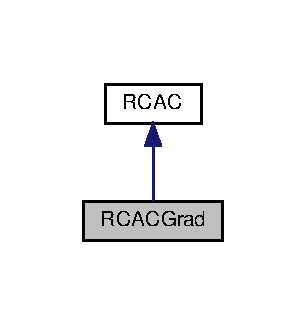
\includegraphics[width=147pt]{class_r_c_a_c_grad__inherit__graph}
\end{center}
\end{figure}


Collaboration diagram for R\+C\+A\+C\+Grad\+:\nopagebreak
\begin{figure}[H]
\begin{center}
\leavevmode
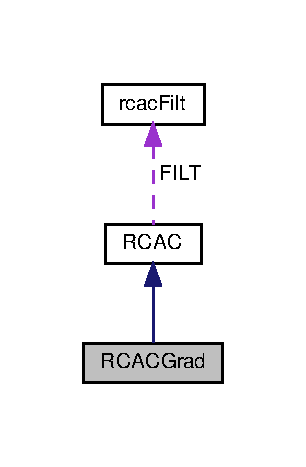
\includegraphics[width=147pt]{class_r_c_a_c_grad__coll__graph}
\end{center}
\end{figure}
\subsection*{Public Member Functions}
\begin{DoxyCompactItemize}
\item 
\hyperlink{class_r_c_a_c_grad_a62f433bc3efdfc5133105c5b2fd59ea6}{R\+C\+A\+C\+Grad} (\hyperlink{structrcac_grad_flags}{rcac\+Grad\+Flags} \&F\+L\+A\+GS, \hyperlink{structrcac_filt}{rcac\+Filt} \&F\+I\+LT)
\end{DoxyCompactItemize}
\subsection*{Additional Inherited Members}


\subsection{Detailed Description}
This class contains the Gradient implementation of \hyperlink{class_r_c_a_c}{R\+C\+AC}. The class contains a constructor and an implementation of the coeff\+Update method. 

\subsection{Constructor \& Destructor Documentation}
\mbox{\Hypertarget{class_r_c_a_c_grad_a62f433bc3efdfc5133105c5b2fd59ea6}\label{class_r_c_a_c_grad_a62f433bc3efdfc5133105c5b2fd59ea6}} 
\index{R\+C\+A\+C\+Grad@{R\+C\+A\+C\+Grad}!R\+C\+A\+C\+Grad@{R\+C\+A\+C\+Grad}}
\index{R\+C\+A\+C\+Grad@{R\+C\+A\+C\+Grad}!R\+C\+A\+C\+Grad@{R\+C\+A\+C\+Grad}}
\subsubsection{\texorpdfstring{R\+C\+A\+C\+Grad()}{RCACGrad()}}
{\footnotesize\ttfamily R\+C\+A\+C\+Grad\+::\+R\+C\+A\+C\+Grad (\begin{DoxyParamCaption}\item[{\hyperlink{structrcac_grad_flags}{rcac\+Grad\+Flags} \&}]{F\+L\+A\+GS,  }\item[{\hyperlink{structrcac_filt}{rcac\+Filt} \&}]{F\+I\+LT }\end{DoxyParamCaption})}

Value constructor for the \hyperlink{class_r_c_a_c_grad}{R\+C\+A\+C\+Grad} class. Required.


\begin{DoxyParams}{Parameters}
{\em F\+L\+A\+GS} & \hyperlink{structrcac_grad_flags}{rcac\+Grad\+Flags} struct containing the flags for the gradient \hyperlink{class_r_c_a_c}{R\+C\+AC} \\
\hline
{\em F\+I\+LT} & base \hyperlink{structrcac_filt}{rcac\+Filt} struct containing the filter coefficients \\
\hline
\end{DoxyParams}


The documentation for this class was generated from the following files\+:\begin{DoxyCompactItemize}
\item 
R\+C\+A\+C\+Grad.\+hpp\item 
R\+C\+A\+C\+Grad.\+cpp\end{DoxyCompactItemize}

\hypertarget{structrcac_grad_flags}{}\section{rcac\+Grad\+Flags Struct Reference}
\label{structrcac_grad_flags}\index{rcac\+Grad\+Flags@{rcac\+Grad\+Flags}}


{\ttfamily \#include $<$R\+C\+A\+C\+Grad.\+hpp$>$}

\subsection*{Public Attributes}
\begin{DoxyCompactItemize}
\item 
\mbox{\Hypertarget{structrcac_grad_flags_aa41af27b85832a58edf4aa1004d5878e}\label{structrcac_grad_flags_aa41af27b85832a58edf4aa1004d5878e}} 
int {\bfseries lz}
\item 
\mbox{\Hypertarget{structrcac_grad_flags_aeec5a48d77bbd2b772a7929ae88240f6}\label{structrcac_grad_flags_aeec5a48d77bbd2b772a7929ae88240f6}} 
int {\bfseries ly}
\item 
\mbox{\Hypertarget{structrcac_grad_flags_a32e588defb7681a51047146f01ffc56a}\label{structrcac_grad_flags_a32e588defb7681a51047146f01ffc56a}} 
int {\bfseries lu}
\item 
\mbox{\Hypertarget{structrcac_grad_flags_abd48ba6b1705024407c404ec1d516fbf}\label{structrcac_grad_flags_abd48ba6b1705024407c404ec1d516fbf}} 
int {\bfseries Nc}
\item 
\mbox{\Hypertarget{structrcac_grad_flags_aa6a7ba7421f33b289a2a83dcc5126824}\label{structrcac_grad_flags_aa6a7ba7421f33b289a2a83dcc5126824}} 
Eigen\+::\+Vector\+Xd {\bfseries theta\+\_\+0}
\item 
\mbox{\Hypertarget{structrcac_grad_flags_a2e8e4e6f5aceab6ad374401323163bc0}\label{structrcac_grad_flags_a2e8e4e6f5aceab6ad374401323163bc0}} 
int {\bfseries filtorder}
\item 
\mbox{\Hypertarget{structrcac_grad_flags_a9d997800d9823660dd77d0a13f07eb1d}\label{structrcac_grad_flags_a9d997800d9823660dd77d0a13f07eb1d}} 
int {\bfseries k\+\_\+0}
\item 
\mbox{\Hypertarget{structrcac_grad_flags_a50b9a7a4eb078317dd355385b5975a18}\label{structrcac_grad_flags_a50b9a7a4eb078317dd355385b5975a18}} 
double {\bfseries alpha}
\end{DoxyCompactItemize}


\subsection{Detailed Description}
This struct contains the basic parameters needed for gradient \hyperlink{class_r_c_a_c}{R\+C\+AC} to work.


\begin{DoxyParams}{Parameters}
{\em lz} & Number of performance measurements \\
\hline
{\em ly} & Number of sensor measurements \\
\hline
{\em lu} & Number of control inputs \\
\hline
{\em Nc} & Controller order \\
\hline
{\em theta\+\_\+0} & Eigen vector with initial controller coefficients. Usually a vector of zeros \\
\hline
{\em filtorder} & Order of the filter ( $G_f$) \\
\hline
{\em k\+\_\+0} & Minimum number of steps to run before starting the controller (usually k\+\_\+0 = Nc) \\
\hline
{\em alpha} & Step size scaling for gradient descent \\
\hline
\end{DoxyParams}


The documentation for this struct was generated from the following file\+:\begin{DoxyCompactItemize}
\item 
R\+C\+A\+C\+Grad.\+hpp\end{DoxyCompactItemize}

\hypertarget{class_r_c_a_c_r_l_s}{}\section{R\+C\+A\+C\+R\+LS Class Reference}
\label{class_r_c_a_c_r_l_s}\index{R\+C\+A\+C\+R\+LS@{R\+C\+A\+C\+R\+LS}}


Inheritance diagram for R\+C\+A\+C\+R\+LS\+:\nopagebreak
\begin{figure}[H]
\begin{center}
\leavevmode
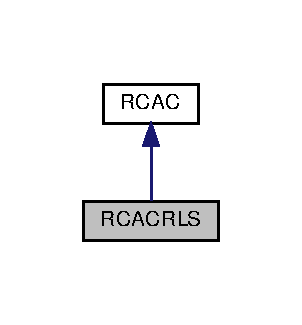
\includegraphics[width=145pt]{class_r_c_a_c_r_l_s__inherit__graph}
\end{center}
\end{figure}


Collaboration diagram for R\+C\+A\+C\+R\+LS\+:\nopagebreak
\begin{figure}[H]
\begin{center}
\leavevmode
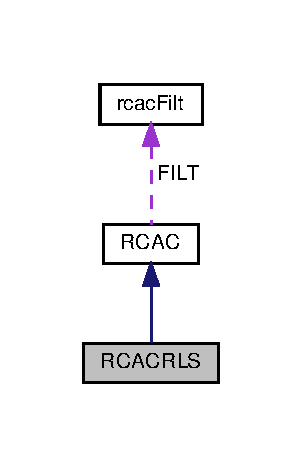
\includegraphics[width=145pt]{class_r_c_a_c_r_l_s__coll__graph}
\end{center}
\end{figure}
\subsection*{Public Member Functions}
\begin{DoxyCompactItemize}
\item 
\mbox{\Hypertarget{class_r_c_a_c_r_l_s_aaac6f50062f37e04d10c40ba55063324}\label{class_r_c_a_c_r_l_s_aaac6f50062f37e04d10c40ba55063324}} 
{\bfseries R\+C\+A\+C\+R\+LS} (\hyperlink{structrcac_rls_flags}{rcac\+Rls\+Flags} \&F\+L\+A\+GS, \hyperlink{structrcac_filt}{rcac\+Filt} \&F\+I\+LT)
\end{DoxyCompactItemize}
\subsection*{Additional Inherited Members}


The documentation for this class was generated from the following files\+:\begin{DoxyCompactItemize}
\item 
R\+C\+A\+C\+R\+L\+S.\+hpp\item 
R\+C\+A\+C\+R\+L\+S.\+cpp\end{DoxyCompactItemize}

\hypertarget{structrcac_rls_flags}{}\section{rcac\+Rls\+Flags Struct Reference}
\label{structrcac_rls_flags}\index{rcac\+Rls\+Flags@{rcac\+Rls\+Flags}}
\subsection*{Public Attributes}
\begin{DoxyCompactItemize}
\item 
\mbox{\Hypertarget{structrcac_rls_flags_a778bf4d0700174efa6deeb624d5bcc09}\label{structrcac_rls_flags_a778bf4d0700174efa6deeb624d5bcc09}} 
int {\bfseries lz}
\item 
\mbox{\Hypertarget{structrcac_rls_flags_a760f93e6bfe4d6669d3671d4f81e814c}\label{structrcac_rls_flags_a760f93e6bfe4d6669d3671d4f81e814c}} 
int {\bfseries ly}
\item 
\mbox{\Hypertarget{structrcac_rls_flags_a39f477577e34ebf3d444871495f197a6}\label{structrcac_rls_flags_a39f477577e34ebf3d444871495f197a6}} 
int {\bfseries lu}
\item 
\mbox{\Hypertarget{structrcac_rls_flags_aca7ebde32128866a43a447f34e92928c}\label{structrcac_rls_flags_aca7ebde32128866a43a447f34e92928c}} 
int {\bfseries Nc}
\item 
\mbox{\Hypertarget{structrcac_rls_flags_abe27441b564ecfdf15fa511275742224}\label{structrcac_rls_flags_abe27441b564ecfdf15fa511275742224}} 
double {\bfseries lambda}
\item 
\mbox{\Hypertarget{structrcac_rls_flags_a8ed42f23cff0f5c333dc453597c0feee}\label{structrcac_rls_flags_a8ed42f23cff0f5c333dc453597c0feee}} 
Eigen\+::\+Vector\+Xd {\bfseries theta\+\_\+0}
\item 
\mbox{\Hypertarget{structrcac_rls_flags_ad1869f6e91f05bb8c80c6559b0c93ac7}\label{structrcac_rls_flags_ad1869f6e91f05bb8c80c6559b0c93ac7}} 
int {\bfseries filtorder}
\item 
\mbox{\Hypertarget{structrcac_rls_flags_a05c788f1af0d4fffffa6aea1be991b0b}\label{structrcac_rls_flags_a05c788f1af0d4fffffa6aea1be991b0b}} 
int {\bfseries k\+\_\+0}
\item 
\mbox{\Hypertarget{structrcac_rls_flags_a2eace0273d4c073088e3116c9b2ddcc5}\label{structrcac_rls_flags_a2eace0273d4c073088e3116c9b2ddcc5}} 
Eigen\+::\+Matrix\+Xd {\bfseries P0}
\item 
\mbox{\Hypertarget{structrcac_rls_flags_a77b15a161e92da2bdd00e07f6c13e3ba}\label{structrcac_rls_flags_a77b15a161e92da2bdd00e07f6c13e3ba}} 
Eigen\+::\+Matrix\+Xd {\bfseries Ru}
\item 
\mbox{\Hypertarget{structrcac_rls_flags_aeef4a3ade42d1d937f09dfaa9b8ce5ba}\label{structrcac_rls_flags_aeef4a3ade42d1d937f09dfaa9b8ce5ba}} 
Eigen\+::\+Matrix\+Xd {\bfseries Rz}
\end{DoxyCompactItemize}


The documentation for this struct was generated from the following file\+:\begin{DoxyCompactItemize}
\item 
R\+C\+A\+C\+R\+L\+S.\+hpp\end{DoxyCompactItemize}

\chapter{File Documentation}
\hypertarget{_r_c_a_c_creator_8hpp}{}\section{R\+C\+A\+C\+Creator.\+hpp File Reference}
\label{_r_c_a_c_creator_8hpp}\index{R\+C\+A\+C\+Creator.\+hpp@{R\+C\+A\+C\+Creator.\+hpp}}
{\ttfamily \#include \char`\"{}R\+C\+A\+C.\+hpp\char`\"{}}\newline
{\ttfamily \#include \char`\"{}R\+C\+A\+C\+R\+L\+S.\+hpp\char`\"{}}\newline
{\ttfamily \#include \char`\"{}R\+C\+A\+C\+Grad.\+hpp\char`\"{}}\newline
Include dependency graph for R\+C\+A\+C\+Creator.\+hpp\+:
\nopagebreak
\begin{figure}[H]
\begin{center}
\leavevmode
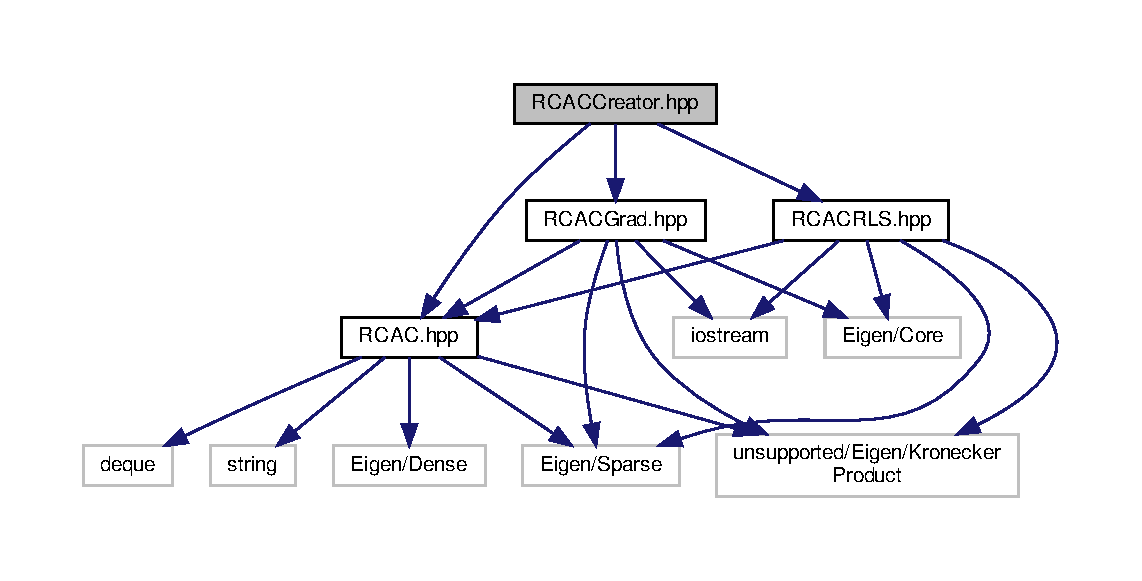
\includegraphics[width=350pt]{_r_c_a_c_creator_8hpp__incl}
\end{center}
\end{figure}
\subsection*{Functions}
\begin{DoxyCompactItemize}
\item 
\mbox{\Hypertarget{_r_c_a_c_creator_8hpp_a7283243a03469a39d685519a92149e57}\label{_r_c_a_c_creator_8hpp_a7283243a03469a39d685519a92149e57}} 
\hyperlink{structrcac_filt}{rcac\+Filt} {\bfseries init\+Filt\+Simulink} (int lz, int ly, int lu, int Nc, int filtorder, double $\ast$\&F\+I\+L\+Tmx)
\item 
\hyperlink{class_r_c_a_c}{R\+C\+AC} $\ast$ \hyperlink{_r_c_a_c_creator_8hpp_ade37a3e8eb11e33b6cad1d31ce1691fe}{init\+Simulink} (double $\ast$\&F\+L\+A\+G\+Smx, double $\ast$\&F\+I\+L\+Tmx, std\+::string \&rcac\+Type)
\end{DoxyCompactItemize}
\subsection*{Variables}
\begin{DoxyCompactItemize}
\item 
\mbox{\Hypertarget{_r_c_a_c_creator_8hpp_ae1ffa3a482052e3f0c2029e14dcc74eb}\label{_r_c_a_c_creator_8hpp_ae1ffa3a482052e3f0c2029e14dcc74eb}} 
std\+::string {\bfseries use\+R\+LS} = \char`\"{}R\+LS\char`\"{}
\item 
\mbox{\Hypertarget{_r_c_a_c_creator_8hpp_a1514da1259b217343d732f38db5afdea}\label{_r_c_a_c_creator_8hpp_a1514da1259b217343d732f38db5afdea}} 
std\+::string {\bfseries use\+Grad} = \char`\"{}Grad\char`\"{}
\end{DoxyCompactItemize}


\subsection{Detailed Description}
Define the methods for initializing different \hyperlink{class_r_c_a_c}{R\+C\+AC} types here


\begin{DoxyParams}{Parameters}
{\em use\+R\+LS} & The flag for the R\+LS based \hyperlink{class_r_c_a_c}{R\+C\+AC} \\
\hline
{\em use\+Grad} & The flag for the Gradient based \hyperlink{class_r_c_a_c}{R\+C\+AC} \\
\hline
\end{DoxyParams}


\subsection{Function Documentation}
\mbox{\Hypertarget{_r_c_a_c_creator_8hpp_ade37a3e8eb11e33b6cad1d31ce1691fe}\label{_r_c_a_c_creator_8hpp_ade37a3e8eb11e33b6cad1d31ce1691fe}} 
\index{R\+C\+A\+C\+Creator.\+hpp@{R\+C\+A\+C\+Creator.\+hpp}!init\+Simulink@{init\+Simulink}}
\index{init\+Simulink@{init\+Simulink}!R\+C\+A\+C\+Creator.\+hpp@{R\+C\+A\+C\+Creator.\+hpp}}
\subsubsection{\texorpdfstring{init\+Simulink()}{initSimulink()}}
{\footnotesize\ttfamily \hyperlink{class_r_c_a_c}{R\+C\+AC}$\ast$ init\+Simulink (\begin{DoxyParamCaption}\item[{double $\ast$\&}]{F\+L\+A\+G\+Smx,  }\item[{double $\ast$\&}]{F\+I\+L\+Tmx,  }\item[{std\+::string \&}]{rcac\+Type }\end{DoxyParamCaption})}

This function takes an array format of the Flags and Filt from M\+A\+T\+L\+AB and converts them to a Eigen compatible matrix/vector.

This must be defined for each type of \hyperlink{class_r_c_a_c}{R\+C\+AC} that is created.

{\bfseries  This function is N\+OT meant to be called outside of R\+C\+A\+C\+Simulink.\+cpp }


\begin{DoxyParams}{Parameters}
{\em F\+L\+A\+G\+Smx} & Array from M\+A\+T\+L\+AB in a special order for the flags (check the source file for the order) \\
\hline
{\em F\+I\+L\+Tmx} & Array from M\+A\+T\+L\+AB in a special order for the filter variables \\
\hline
{\em F\+I\+LT} & \hyperlink{class_r_c_a_c}{R\+C\+AC} type taken from a matlab char string (C-\/style) and converted to a string (C++ string) \\
\hline
\end{DoxyParams}

%--- End generated contents ---

% Index
\backmatter
\newpage
\phantomsection
\clearemptydoublepage
\addcontentsline{toc}{chapter}{Index}
\printindex

\end{document}
